\documentclass[11pt]{article}
\usepackage[utf8]{inputenc}
\usepackage[T1]{fontenc}
\usepackage[french]{babel}
\usepackage{amsmath, amsfonts, amssymb}
\usepackage{verbatim}
\usepackage{amsthm}
\usepackage{geometry}
\usepackage{array}
\usepackage{caption}
\usepackage{graphicx}
\usepackage{float} 
\usepackage{hyperref}
\usepackage{adjustbox}
\usepackage{nomencl}
\usepackage[]{algorithm2e}


% taille des marges
\geometry{hmargin=2cm,vmargin=2.5cm}

\title{Absorbing Boundary Layers in Time Domain Elastodynamics: Two-Dimensional Perfectly Matched Layer}
\author{Poulain Alexandre}
\date{\today}
\def\doubleunderline#1{\underline{\underline{#1}}}


\begin{document}
\pagestyle{empty}
\begin{titlepage}
\begin{sffamily}
\begin{center}
    \vspace*{2cm}
    \noindent\hrulefill \\
    \vspace*{1cm}
    {\huge \bfseries Perfectly Matched Layers 1D}\\[0.5cm]
    {\huge  \itshape Semester Project} \\[0.5cm]
    {\large Laboratoire de simulation en mécanique des solides (LSMS)}\\[0.5cm]
    {\large Ecole Polytechnique Fédérale de Lausanne 2017-2018}\\[1cm]
    
    March 2018 - August 2018 \\[1cm]
    \noindent\hrulefill 
    \vspace{2cm}
    


      
\includegraphics{images/EPFL-Logo.jpg}\\[1cm]
      

    \emph{Student:} Alexandre \textsc{Poulain}\\[1cm]
    \emph{Project supervisor:} Michael \textsc{Brun}\\[1cm]
    \emph{Laboratory director:} Jean-François \textsc{Molinari}

    
    
    \vfill{\large January 2018}

\end{center}
\end{sffamily}
\end{titlepage}

\newpage
\renewcommand{\abstractname}{Abstract}
\begin{abstract}
%% Background (short)
% What is known
Absorbing boundary layers is a common method to solve numerically wave propagation phenomena in infinite or unbounded domains. Several techniques exist to construct these boundaries such as the introduction of Rayleigh damping in the absorbing layer or as presented in this report, perfectly matched layers (PML). They find their application in many fields such as electromagnetism and elastodynamics.   
% What is not known
Due to the complexity of the formulation of these PMLs, their construction and use remain a challenge. A large number of formulations and implementations have been proposed through the years to tackle some problems such as instability and performance.  
%% Methods (long)
% What was done
We attend in this report to present the formulation of a stable unsplit field two-dimensional perfectly matched layer based on the weak form of the equations of elastodynamics. 

\noindent First of all, the presentation of the construction of the PML will be detailed, including an extensive description of the governing equations. Using this description, we will explain the proof of the stability of the numerical scheme: the method employed will be described and the results will be analyzed. This stability analysis will be followed by the implementation of the scheme in Akantu: an open-source finite-element software developed at the Computational Solid Mechanics Laboratory of the EPFL. The results on two test cases will be reviewed in the second part and a special attention will be dedicated to the reflection of the waves since this parameter represents the efficiency of the PML. We will shortly see that the scheme is efficient to attenuate incident waves with less than $1$ percent of the incident wave reflected in some extreme cases where the length of the PML and the coefficients of the attenuation functions are reduced to their minimum.   
%% Results


%% Conclusions




\end{abstract}


\newpage

\tableofcontents

\newpage
\makenomenclature
 
\mbox{}
 
\nomenclature{$c_s$}{S-wave velocity}
\nomenclature{$E$}{Young modulus}
\nomenclature{$\sigma$}{Stress}
\nomenclature{$\epsilon$}{Strain}
\nomenclature{$u$,$\Dot{u}$,$\Ddot{u}$}{Displacement, velocity and acceleration}
\nomenclature{$\lambda(x)$}{Stretching function}
\nomenclature{$f^p$, $f^e$}{Damping functions}
\nomenclature{$L$,$L_p$}{Length of medium, length of PML}
\nomenclature{$\omega$}{Frequency of excitation}
\nomenclature{$L_e$}{Element length}
 
\printnomenclature

\newpage

\section{Introduction}
\subsection{Absorbing boundaries}
\begin{frame}{Absorbing boundaries}
    \begin{itemize}[<+->]
        \item Common practice to solve numerically wave propagation on unbounded domains.
        \item Important topic for many research and engineering applications.
        \item Simulation of earthquake ground motion, for soil-structure, geophysical, subsurface sensing, waveguides problems.
        \pause
        \vspace{0.7cm}
        \item 2 kinds of method:
        \begin{itemize}
            \item \underline{Absorbing boundary conditions :} specific conditions at the model boundaries.
        \pause
            \item \underline{Absorbing boundary layers (ABL) :} layer surrounding the domain of interest.
        \end{itemize}    
    \end{itemize}
\end{frame}

\subsection{Perfectly matched layers}
\begin{frame}{Perfectly matched layers}
\pause
    \begin{itemize}
        \item \underline{split-field PML:} 
        \begin{itemize}
        \pause
            \item Introduced by Bérenger in the context of electromagnetics.
            \item Extended by Hastings et al to elastodynamics.
            \item Use on complex-valued coordinate stretching.
            \item Field splitting: partition of the variables into two components parallel and perpendicular to the truncation boundary.
        \end{itemize}
    \item \underline{unsplit-field PML:} 
        \begin{itemize}
        \pause
            \item Introduced by Wang in the context of elastodynamics (CPML) $\rightarrow$ \textcolor{red}{Complexity} 
            \pause
            \item Basu and Chopra: unsplit-field PML for time-harmonic elastodynamics. $\rightarrow$ \textcolor{green}{finite-element implementation}
        \end{itemize}
    \end{itemize}
\end{frame}

\begin{frame}{Stability of PML in the literature}
\pause
    \begin{itemize}
        \item \underline{split-field PML:} 
        \begin{itemize}
        \pause
        	\item Stability analysis using Slowness diagrams and wave fronts.
        	\item Definitions of sufficiant and necessary conditions of stability [Becache 2006]. 
            \item First order finite difference discretization: Prone to instability in anisotropic media.
            \item Second order discretization: stable [Duru-2012]

        \end{itemize}
    \item \underline{unsplit-field PML:} 
        \begin{itemize}
        \pause
            \item Stability proved for electromagnetics (Maxwell's equations) [Bécache 2004].
            \pause
            \item In the context of elastic wave propagation problems: no much publications.
        \end{itemize}
    \end{itemize}
\end{frame}


\newpage
\section{Description}
%%%%%%
% Maybe a part here on how to make the junction GC maybe 

\subsection{Elastic medium}
As an introduction of the governing equations, let us describe the elastic medium since the PML is surrounding it. In fact the construction of the PML relies on the same governing equations as the physical medium and share some parameters with it.\\
Let us consider an isotropic homogeneous elastic medium under plane-strain motion and without body forces. The motion in the medium is governed by:
\begin{equation}
\begin{cases}
\sum_{j} \frac{\partial \sigma_{ij}}{\partial x_j} & =  \rho \ddot{u}_i \\
\sigma_{ij} &= \sum_{k,l} C_{ijkl} \epsilon_{kl} \\
\epsilon_{ij} &= \frac{1}{2} \left(\frac{\partial u_{i}}{\partial x_j} + \frac{\partial u_{j}}{\partial x_i} \right)
\end{cases}
\label{eq:2D-motion-elastic}
\end{equation} 
With $u(x,t)$ the displacement, $\epsilon$ the strain, $\sigma$ the stress, $\rho$ the mass density of the medium. $C$ is the material stiffness tensor and its components are expressed in term of the Kronecker delta $\delta_{ij}$:
\begin{equation}
C_{ijkl} = (\kappa-\frac{2}{3}\mu)\delta_{ij}\delta_{kl}+\mu(\delta_{ik}\delta_{jl} + \delta_{il} \delta_{jk})
\end{equation} 
Where $\kappa$ is the bulk modulus and $\mu$ the shear modulus.\\
If we consider an unbounded domain, the system \ref{eq:2D-motion-elastic} admits solutions of the form of P- waves and S-waves. The solutions of P-waves have the following formulation: 
\begin{equation}
u(x,t) = q \exp(-i k_p x . p) \exp(i\omega t)
\label{eq:elastic-sol-p}
\end{equation}
with $k_p = \frac{\omega}{c_p}$ where $\omega$ is the frequency of the wave and $c_p = \sqrt{(\kappa+4\mu/3)/\rho}$ which is the celerity of the P-wave. In the equation \ref{eq:elastic-sol-p} $p$ denotes the unit vector pointing in the direction of propagation of the wave and $q=\pm p$.   
The solution of S-wave form take the following formulation:
\begin{equation}
u(x,t) = q \exp(-i k_s x.p) \exp(i \omega t)
\end{equation}
Where $k_s = \omega / c_s$ and the S-wave speed is $c_s =\sqrt{ \mu/\rho}$ and $q.p =0$.
\subsection{Strong form in frequency domain}
Before describing the governing equations of the two-dimensional PML let us introduce the following notations: $\Omega_{PML}$ will denote the PML domain which is bounded by $\Gamma_{PML} = \Gamma_{PML}^D \cup \Gamma_{PML}^N$. $\Gamma_{PML}^D$ corresponds to the boundary where the Dirichlet condition are applied (imposed displacement). $\Gamma_{PML}^N$ is the boundary where the tractions are applied and represents the boundary of the Neumann conditions. The intersection of these two boundaries defined by the imposed conditions is null: $\Gamma_{PML}^D \cap \Gamma_{PML}^N = \emptyset$. The temporal domain will be denoted by $J = [0,T]$ with $T$ the end time.\\
The classical formulation of PML begins with the introduction of the complex-valued coordinates stretching functions $\lambda_i$. They are used to replace the real coordinates by the complex ones: $x_i \rightarrow \tilde{x}_i: \mathbb{R} \rightarrow \mathbb{C}$.
\begin{equation}
\lambda_i(x_i) = \frac{\partial \tilde{x}_i}{\partial x_i} = 1+f^e_i(x_i)-\frac{i}{b k_s} f^p_i(x_i)
\label{eq:complex-stret-2D}
\end{equation} 
where $b$ is the characteristic length of the problem. $k_s=\omega / c_s$ denotes the wavenumber ($\omega$ is the pulsation and $c_s$ is the celerity of shear waves). $i$ is used to denote the direction $x$ or $y$. $f^p_i$ and $f^e_i$ are the attenuation functions for respectively propagating and evanescent waves. They are written as a polynomial of order $n$. 
\begin{equation}
f^\alpha_i = a_\alpha \left(\frac{x_i - x_0}{L_{p,i}}  \right), x_i \in [x0,x0+d] \\
\label{eq:attenuation-functions}
\end{equation}
% Little explanation of what is the effect of the coordinate stretching function ? 
The tunable property of the PML relies mainly on the formulation of the attenuation functions. The value of the coefficients of attenuation $a_p$, $a_e$, the order of the polynomial $n$, and the size of the PML $L_p$ can be defined by the user. As we will see in the section concerning the numerical results, these parameters need to be chosen carefully and depending on the problem to obtain the "best" result possible. The concept of "best result" depends on the expectations of the user. Accuracy versus performance is a deep-seated problem for all numerical simulations. The perfectly matched layer does not get out of this rule. In order to choose the value of these coefficients, we can use the reflection coefficient for an incident pressure wave given by \cite{Basu2004}:
\begin{equation}
R_{pp} = \frac{cos(\theta+\theta_s)}{cos(\theta-\theta_s)} \exp\left[-2\frac{c_s}{c_p}F_1(L_p)cos(\theta)\right]
\label{eq:Rpp} 
\end{equation} 
Where $c_p$ stands for the velocity of P-waves. The incident P-wave is characterised by $\theta$, its angle of incidence and $\theta_s$, its reflective angle after being reflected at the end of the PML. $F_1$ corresponds to the integral over the PML of the attenuation function for propagating waves: $F_1(L_p) = \int_{s=0}^{L_p} f^p(s) ds = \frac{\beta_0 L_p}{n+1}$. Thus, the attenuation coefficients can be expressed in function of the reflection coefficient:
\begin{equation}
a_\alpha = \ln\left(\frac{cos(\theta+\theta_s)}{R_{pp}cos(\theta-\theta_s)} \right) \frac{c_p}{c_s} \frac{n+1}{L_p cos(\theta)}
\label{eq:alpha_kucu}
\end{equation} 
If we consider that the incident wave has an angle of $\theta = \theta_s = 0$ therefore the value of the coeffecient has the form:
\begin{equation}
a_\alpha = \ln\left(\frac{1}{R_{pp}} \right) \frac{c_p}{c_s} \frac{n+1}{L_p cos(\theta)}
\end{equation}
\par Using the complex-valued coordinates stretching functions \ref{eq:complex-stret-2D}, the strong form of the equations of motion for the PML in the frequency domain is defined by:
\begin{equation}
\begin{cases}
\sum_{j} \frac{1}{\lambda_j(x_j)} \frac{\partial \sigma_{ij}}{\partial x_j} & = - \omega^2 \rho u_i \\
\sigma_{ij} &= \sum_{k,l} C_{ijkl} \epsilon_{kl} \\
\epsilon_{ij} &= \frac{1}{2} \left(\frac{1}{\lambda_j(x_j)} \frac{\partial u_{i}}{\partial x_j} + \frac{1}{\lambda_i(x_i)} \frac{\partial u_{j}}{\partial x_i} \right)
\end{cases}
\label{eq:2D-PML-freq}
\end{equation} 
Where $C_{ijkl}$ are the components of the elastic constitutive tensor. In fact the system \ref{eq:2D-PML-freq} defines a perfectly matched medium (PMM) and the elastic medium is just a specific case of PMM with $\lambda_j(x_j) = 1$, $\forall x \in \Omega_{PML}$. If we imagine a PML, surrounding an elastic medium, as in the figure \ref{fig:scheme-layers}, we have to define for the PML $\lambda_j(x_j) = 1$ for $\forall x \in \Gamma_{PML}$ at the interface between the two-subdomains. \\
The system of equations \ref{eq:2D-PML-freq} assumes harmonic time-dependence of the displacement, stress and strain. Therefore, its solution can be written as $u(x,t) = \overline{u}(x,t)exp(i \omega t)$. If the stretching functions have the formulation \ref{eq:complex-stret-2D} then the system \ref{eq:2D-PML-freq} has solutions of the form: 
\begin{equation}
\overline{u}(x) = \exp[-\frac{c_s}{c_p}\sum_i F_i(x_i)p_i ] q  \exp(i k_p x . p)
\end{equation}
with $q = \pm p$, and
\begin{equation}
\overline{u}(x) = \exp [ -\sum_i F_i(x_i)p_i ] q  \exp(- i k_s x . p)
\end{equation}
with $q.p=0$ and $F_i(x_i) = \int_0^{x_i} f_i(\xi) d\xi$.\\
Therefore the solution admitted in the PML corresponds to the solution of the system \ref{eq:2D-motion-elastic} but with an imposed spatial attenuation. 
The attenuation contained in the term $\exp[ - F_i p_i ]$ for the direction $i$ is independent of the frequency if the direction of propagation is. 


\begin{figure}[H]
\centering
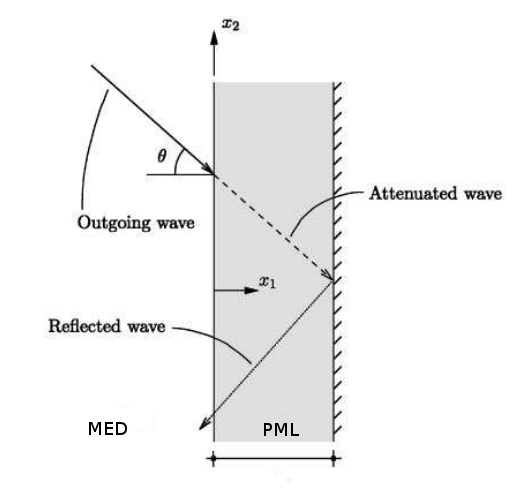
\includegraphics[scale=0.5]{images/scheme-layers.png}
\caption{Scheme of the propagation of a wave within the elastic medium (on the left) and the PML (on the right)}
\label{fig:scheme-layers}
\end{figure} 
\subsection{Strong form in time domain}
\par The strong form of the PML in the temporal domain can be obtained by inverse Fourier transform of each equation of \ref{eq:2D-PML-freq}. Indeed the introduction of the complex-valued coordinates stretching functions makes the application of this inverse easier. In the following equation the number of lines below a tensor will specify its order. 
%% Explanation on how to obtain these equations (for final version) maybe in appendice
\begin{equation}
\begin{cases}
div(\doubleunderline{\sigma}\tilde{F}^e + \doubleunderline{\Sigma}\tilde{F}^p) = \rho f_m \underline{\ddot{u}} + \rho \frac{c_s}{b} f_c \underline{\dot{u}} + \frac{\mu}{b^2}f_k \underline{u}, & \text{In } \Omega_{PML} \times J\\
\doubleunderline{\sigma} =  C : \doubleunderline{\epsilon} , & \text{In } \Omega_{PML} \times J\\
F^{eT} \doubleunderline{\dot{\epsilon}}F^e + F^{pT}\underline{\epsilon}F^e + F^{eT}\doubleunderline{\epsilon}F^p + F^{pT} \doubleunderline{E} F^p = ...\\
\frac{1}{2}(\nabla \underline{\dot{u}}^T F^e + F^{eT} \nabla \underline{\dot{u}})+\frac{1}{2}(\nabla \underline{u}^T F^p + F^{pT} \nabla \underline{u}), & \text{In } \Omega_{PML} \times J\\
\end{cases}
\label{eq:2D-PML-strong-timeD}
\end{equation}
submitted to the homogeneous boundary conditions:
\begin{equation}
\begin{cases}
\underline{u}=0,& \text{on } \Gamma_{PML}^D\\
(\doubleunderline{\sigma}\tilde{F}^e + \doubleunderline{\Sigma}\tilde{F}^p).n , & \text{on } \Gamma_{PML}^N 
\end{cases}
\label{eq:conditions-lim}
\end{equation}
Let us now summarize the form of the different matrices $F^e,F^p,\tilde{F}^e$ and $\tilde{F}^p$ of the above equations.
\begin{equation}
F^e = \begin{bmatrix}
1+f^e_1(x1)&0\\0&1+f^e_2(x2)
\end{bmatrix}, F^p = \begin{bmatrix}
\frac{c_s}{b}f^p_1(x1)&0\\0&\frac{c_s}{b}f^p_2(x2) 
\end{bmatrix} 
\end{equation}
\begin{equation}
\tilde{F}^e = \begin{bmatrix}
1+f^e_2(x2)&0\\0&1+f^e_1(x1)
\end{bmatrix}, \tilde{F}^p = \begin{bmatrix}
\frac{c_s}{b}f^p_2(x2)&0\\0&\frac{c_s}{b}f^p_1(x1) 
\end{bmatrix} 
\end{equation}
Let us now focus on the first equation of \ref{eq:2D-PML-strong-timeD}, the functions $f_m$, $f_c$ and $f_k$ depend on the attenuation functions:
\begin{equation}
\begin{cases}
f_m = (1+f^e_1(x1))(1+f^e_2(x2))\\
f_c = (1+f^e_1(x1))f^p_2(x2) + (1+f^e_2(x2))f^p_1(x1)\\
f_k = f^p_1(x_1)f^p_2(x_2)
\end{cases}
\end{equation}
The next elements to define, which appear in the first and the third equations of \ref{eq:2D-PML-strong-timeD} are the integral of the stress and the strain.
\begin{equation}
\doubleunderline{\Sigma} = \int^t_0 \doubleunderline{\sigma} dt, \doubleunderline{E} = \int^t_0 \doubleunderline{\epsilon} dt
\end{equation} 
\subsection{Displacement-based weak form}
Let us introduce the test function $\underline{v}$ belonging to an admissible space of solution $V$. Premultiplying the first equation of the strong form \ref{eq:2D-PML-strong-timeD} by $\underline{v}$ and integrating over the PML domain gives :
\begin{align}
\int_{\Omega_{PML}} \underline{v}.div(\doubleunderline{\sigma}\tilde{F}^e + \doubleunderline{\Sigma}\tilde{F}^p) d\Omega_{PML} & = \int_{\Omega_{PML}} \rho f_m \underline{v}.\underline{\ddot{u}} d\Omega_{PML} + ... \nonumber\\
&  \int_{\Omega_{PML}} \rho \frac{c_s}{b} f_c \underline{v}.\underline{\dot{u}} d\Omega_{PML} +  \int_{\Omega_{PML}} \frac{\mu}{b^2}f_k \underline{v}. \underline{u}  d\Omega_{PML},  \text{In } \Omega_{PML} \times J 
\label{eq:weak-form-motion}
\end{align}
Using the Gauss divergence theorem and integration per parts gives:

\begin{multline}
\int_{\Gamma_{PML}} \underline{v} .\left(\doubleunderline{\sigma}\tilde{F}^e + \doubleunderline{\Sigma}\tilde{F}^p \right).\underline{n} d\Gamma_{PML}  = \int_{\Omega_{PML}} \rho f_m \underline{\ddot{u}} . \underline{v} d\Omega_{PML} + ... \nonumber\\
\int_{\Omega_{PML}} \rho \frac{c_s}{b} f_c \underline{\dot{u}} . \underline{v} d\Omega_{PML} +  \int_{\Omega_{PML}} \frac{\mu}{b^2}f_k \underline{u} . \underline{v} d\Omega_{PML} +\int_{\Omega_{PML}} \doubleunderline{\tilde{\epsilon}}^e : \doubleunderline{\sigma} d\Omega_{PML} + \int_{\Omega_{PML}} \doubleunderline{\tilde{\epsilon}}^p : \doubleunderline{\Sigma} d\Omega_{PML},  \text{In } \Omega_{PML} \times J
\end{multline}
$\underline{n}$ is the vector normal to the boundary of the PML $\Gamma_{PML}$. The tensors $\doubleunderline{\tilde{\epsilon}}^p$ and $\doubleunderline{\tilde{\epsilon}}^e$ depend on the attenuation functions:
\begin{equation}
\begin{cases}
\doubleunderline{\tilde{\epsilon}}^e = \frac{1}{2}\left(\nabla \underline{v} \tilde{F}^e + \tilde{F}^{eT} \nabla \underline{v}^T  \right) \\
\doubleunderline{\tilde{\epsilon}}^p = \frac{1}{2}\left(\nabla \underline{v} \tilde{F}^p + \tilde{F}^{pT} \nabla \underline{v}^T  \right)
\end{cases}
\label{eq:weak-first-eq}
\end{equation}
Using the weak form of the equation of motion within the PML in the temporal domain \ref{eq:weak-form-motion} we can define the mass, damping and stiffness matrices:
\begin{equation}
m^{e} = \int_{\Omega_e} \rho f_m N_I N_J d\Omega_e I_d
\label{eq:2Dpml-elem-mass}
\end{equation}
\begin{equation}
 c^{e} = \int_{\Omega_e} \rho f_c \frac{c_s}{b} N_I N_J d\Omega_e I_d
 \label{eq:2Dpml-elem-damp}
\end{equation}
\begin{equation}
  k^{e} = \int_{\Omega_e} \frac{\mu}{b^2} f_k N_I N_J d\Omega_e I_d 
  \label{eq:2Dpml-elem-stiff}
\end{equation}
In the above equation $N_I$ is the nodal shape function for node $I$.
Let us introduce a notation for the internal forces term: 
\begin{equation}
p^e = \int_{\Omega_{PML}} \doubleunderline{\tilde{\epsilon}}^e : \doubleunderline{\sigma} d\Omega_{PML} + \int_{\Omega_{PML}} \doubleunderline{\tilde{\epsilon}}^p : \doubleunderline{\Sigma} d\Omega_{PML}
\end{equation}
In order to modify this term we need to make a temporal discretization.
\subsection{Complete discrete form}
Before describing the complete discrete equations of two-dimensional PML featuring the discretization in space and time, we need to introduce the following notation. The hat notation above an element will specify that the tensor is written in Voigt notation. For example $\hat{\sigma} = \begin{pmatrix}
\sigma_{11} \\
\sigma_{22} \\
\sigma_{12}
\end{pmatrix}$ 
Thus, using a simple temporal discretization with $dt=t_{n+1} - t_n$ we can rewrite the internal forces at time $t_{n+1}$ as:
\begin{equation}
p_{n+1}^e = \int_{\Omega_e} \tilde{B}^{eT} \hat{\sigma}_{n+1} d\Omega_e + \int_{\Omega_e}\tilde{B}^{pT} \hat{\Sigma}_{n+1} d\Omega_e
\label{eq:intern-forces-discrete}
\end{equation} 
The two matrices $\tilde{B}^{p}$ and $\tilde{B}^{e}$ in \ref{eq:intern-forces-discrete} depend on the nodal shape functions and the attenuation functions. They are expressed in term of their nodal submatrices as:
\begin{equation}
\tilde{B}^e_I = \begin{bmatrix}
\tilde{N}^e_{I1}&0\\0&\tilde{N}^e_{I2}\\\tilde{N}^e_{I2}&\tilde{N}^e_{I1}
\end{bmatrix}, \tilde{B}^p_I = \begin{bmatrix}
\tilde{N}^p_{I1}&0\\0&\tilde{N}^p_{I2}\\\tilde{N}^p_{I2}&\tilde{N}^p_{I1}
\end{bmatrix}
\end{equation} 
with 
\begin{equation}
\tilde{N}^e_{Ii} = \tilde{F}^e_{ji}N_{I,j}, \tilde{N}^p_{Ii} = \tilde{F}^p_{ji}N_{I,j}
\end{equation}
And
\begin{equation}
\tilde{B}^T = \tilde{B}^{eT}+dt \tilde{B}^{pT}
\end{equation}
\begin{equation}
B^\epsilon_I = \begin{bmatrix}
F^\epsilon_{11}N^I_{I1}&F^\epsilon_{21}N^I_{I1}\\
F^\epsilon_{12}N^I_{I2}&F^\epsilon_{22}N^I_{I2}\\
F^\epsilon_{11}N^I_{I2}+F^\epsilon_{12}N^I_{I1}& F^\epsilon_{21}N^I_{I2}+F^\epsilon_{22}N^I_{I1}
\end{bmatrix}
\end{equation}
Some assumptions have to be made to perform time stepping. To evaluate the integral of the stress or strain at the next time step we will assume that:
\begin{equation}
\begin{cases}
\hat{\Sigma}_{n+1} &= \hat{\Sigma}_n + dt \hat{\sigma}_{n+1} \\
\hat{E}_{n+1} &= \hat{E}_n + dt \hat{\epsilon}_{n+1}
\end{cases}
\end{equation}
Thus using this assumption, the internal forces term can be rewrite as:
\begin{equation}
p_{n+1}^e = \int_{\Omega_e} \tilde{B}^{T} \hat{\sigma}_{n+1} d\Omega_e + \int_{\Omega_e}\tilde{B}^{pT} \hat{\Sigma}_{n} d\Omega_e
\end{equation}
where
\begin{equation}
\tilde{B}^{T} = \tilde{B}^{eT} + dt \tilde{B}^{pT}
\end{equation}
An additional assumption has to be made to evaluate the derivative of the strain:
\begin{equation}
\dot{\epsilon}_{n+1} = \frac{\epsilon_{n+1}-\epsilon_n}{dt}
\end{equation} 
This corresponds to the first order approxiation due to Taylor's theorem.
Using this assumption in the third equation of \ref{eq:2D-PML-strong-timeD}, the expression of the strain for the next time step can be obtained.
\begin{equation}
\hat{\epsilon}_{n+1} = \frac{1}{dt}\left(B^\epsilon \dot{U}_{n+1} + B^Q U_{n+1} + \frac{1}{dt} \hat{F}^\epsilon \hat{\epsilon}_n - \hat{F}^Q \hat{E}_n\right)
\label{eq:strain-n+1}
\end{equation} 
The matrices $B^\epsilon$, $B^Q$, $\hat{F}^\epsilon$ and $\hat{F}^Q$ depend on the attenuation and the nodal shape functions. The are defined by their nodal submatrices as:
\begin{equation}
B^\epsilon_I = \begin{bmatrix}
F^\epsilon_{11}N^I_{I1}&F^\epsilon_{21}N^I_{I1}\\
F^\epsilon_{12}N^I_{I2}&F^\epsilon_{22}N^I_{I2}\\
F^\epsilon_{11}N^I_{I2}+F^\epsilon_{12}N^I_{I1}& F^\epsilon_{21}N^I_{I2}+F^\epsilon_{22}N^I_{I1}
\end{bmatrix}
\end{equation}
with
\begin{equation}
N^I_{Ii} = F^I_{ij}N_{I,j}
\end{equation}
\begin{equation}
F^I = \left[ F^p+\frac{F^e}{dt} \right]^{-1}, F^\epsilon = F^eF^I, F^Q=F^pF^I
\end{equation}
and
\begin{equation}
\hat{F}^\epsilon_I = \begin{bmatrix}
(F^\epsilon_{11})^2&(F^\epsilon_{21})^2& F^\epsilon_{11}F^\epsilon_{21}\\
(F^\epsilon_{12})^2&(F^\epsilon_{22})^2&F^\epsilon_{12}F^\epsilon_{22}\\
2F^\epsilon_{11}F^\epsilon_{12}&2 F^\epsilon_{21}F^\epsilon_{22}& F^\epsilon_{11}F^\epsilon_{22}+F^\epsilon_{12}F^\epsilon_{21}
\end{bmatrix}
\end{equation}
To obtain the relations for $B^Q$ and $\hat{F}^Q$ the only thing to replace is the superscript $\epsilon$ by $Q$. 
\par The stress $\hat{\sigma}_{n+1}$ is computed using the second equation of \ref{eq:2D-PML-strong-timeD} involving the elastic constitutive tensor $C$. Thus the internal forces term can be expressed in function of the strain and not the stress.
\begin{equation}
p_{n+1}^e = \int_{\Omega_e} \tilde{B}^{T} D \hat{\epsilon}_{n+1} d\Omega_e + \int_{\Omega_e}\tilde{B}^{pT} \hat{\Sigma}_{n} d\Omega_e
\end{equation} 
and using the relation \ref{eq:strain-n+1} this expression can be rewrite as:
\begin{align}
p_{n+1}^e &= \int_{\Omega_e} \tilde{B}^{T} D \left[\frac{1}{dt}\left(B^\epsilon \dot{U}_{n+1} + B^Q U_{n+1} + \frac{1}{dt} \hat{F}^\epsilon \hat{\epsilon}_n - \hat{F}^Q \hat{E}_n\right)  \right] d\Omega_e + \int_{\Omega_e}\tilde{B}^{pT} \hat{\Sigma}_{n} d\Omega_e \\
&= \tilde{c}^e \dot{U}^e_{n+1} + \tilde{k}^e U^e_{n+1} + P(\hat{\epsilon}_n,\hat{E}_n,\hat{\Sigma}_n)
\end{align} 
where 
\begin{equation}
P(\hat{\epsilon}_n,\hat{E}_n,\hat{\Sigma}_n) = \int_{\Omega_e} \tilde{B}^T \frac{D}{dt} \left[\frac{1}{dt}\hat{F}^{\epsilon} \hat{\epsilon} - \hat{F}^Q \hat{E}_n \right] + \tilde{B}^p \hat{\Sigma}_n d\Omega_e
\label{eq:pseudo-intern}
\end{equation}
and 
\begin{equation}
\tilde{c}^{e} = \frac{1}{dt} \int_{\Omega_e} \tilde{B}^T D B^\epsilon d\Omega_e
\label{eq:2Dpml-elem-effdamp}
\end{equation}
\begin{equation}
\tilde{k}^{e} = \frac{1}{dt} \int_{\Omega_e} \tilde{B}^T D B^Q d\Omega_e
\label{eq:2Dpml-elem-effstiff}
\end{equation}
Under the plane-strain assumption the material constitutive matrix is expressed as:
\begin{equation}
\begin{pmatrix}
K+\frac{4}{3}\mu_L& K-\frac{2}{3}\mu_L&0\\
K-\frac{2}{3}\mu_L&K+\frac{4}{3}\mu_L&0\\
0&0&\mu_L
\end{pmatrix}
\end{equation}
Therefore using the above equation we can rewrite \ref{eq:weak-first-eq} as:
\begin{equation}
M\ddot{U}_{n+1} + \left(C+\tilde{C}\right)\dot{U}_{n+1} + \left(K+\tilde{K}\right)U_{n+1} + P(\hat{\epsilon}_n,\hat{E}_n,\hat{\Sigma}_n) = F_{ext}
\label{eq:2Dpml-discrete-motion}
\end{equation}
Where $M$,$C$ and $K$ are respectively the mass, damping and stiffness matrices resulting from the assembly of their element matrices \ref{eq:2Dpml-elem-mass}, \ref{eq:2Dpml-elem-damp} and \ref{eq:2Dpml-elem-stiff}. The matrices $\tilde{K}$ and $\tilde{C}$ derive from the assembly procedure of their element matrices \ref{eq:2Dpml-elem-effstiff} and \ref{eq:2Dpml-elem-effdamp}. $P(\hat{\epsilon}_n,\hat{E}_n,\hat{\Sigma}_n)$ is given by the equation \ref{eq:pseudo-intern} and is known at the beginning of the time step since it depends only on components of the previous time. 
\subsection{Time integration scheme}
The complete discrete equations obtained in the previous part can be integrated using the Newmark-$\beta$ scheme. The classical Newmark approximation formulas are expressed in acceleration form:
\begin{equation}
\begin{cases}
U_{n+1} = U_{n,p} + \beta dt^2 \ddot{U}_{n+1} \\
\dot{U}_{n+1} = \dot{U}_{n,p} + \gamma dt \ddot{U}_{n+1}
\end{cases}
\label{eq:newmark1}
\end{equation}
where the predictors $U_{n,p}$ and $\dot{U}_{n,p}$ have the form:
\begin{equation}
\begin{cases}
U_{n,p} = U_n + dt \dot{U}_n + dt^2 \left(\frac{1}{2} -\beta  \right)\ddot{U}_n \\
\dot{U}_{n,p} = \dot{U}_n + dt (1-\gamma)\ddot{U}_n
\end{cases}
\label{eq:newmark2}
\end{equation}
Substituting the equations \ref{eq:newmark1} and \ref{eq:newmark2} into the discrete form of the equation of motion \ref{eq:2Dpml-discrete-motion} the acceleration at time $t_{n+1}$ can be obtained.
\begin{equation}
\tilde{M}\ddot{U}_{n+1} = F_{ext} - \left(C+\tilde{C}\right)\dot{U}_{n,p} - \left(K+\tilde{K}\right)U_{n,p} - P(\hat{\epsilon}_n,\hat{E}_n,\hat{\Sigma}_n)
\end{equation}
where 
\begin{equation}
\tilde{M} = M + \gamma dt \left(C+\tilde{C}\right) + \beta dt^2 \left(K+\tilde{K}\right)
\end{equation}
This matrix needs to be inverted, this will be done before beginning the time stepping since all the matrices constituting it remain constant through the time stepping. Two schemes will be used in the following of this report:
\begin{itemize}
\item Implicit Newmark scheme: with $\gamma = 1/2$ and $\beta = 1/4$.
\item Explicit Newmark scheme: with $\gamma = 1/2$ and $\beta = 0$.
\end{itemize} 
The properties of each scheme will be investigated in the next section concerning the stability and the last part will highlight the differences in term of performance and accuracy.\\
Let us summarise the different steps in the following algorithm:
\begin{algorithm}
\caption{PML algorithm}
\begin{algorithmic} 
\REQUIRE Calculate global matrices: $M$, $C$, $K$.
\REQUIRE Calculate: $\tilde{M}^{-1} = \left[ M+ \gamma h C +\beta h^2 K  \right]^{-1}$
\REQUIRE Calculate constant matrices to update internal forces for PML.
\WHILE{not end time} 
\FOR{each element} 
\STATE $P(\hat{\epsilon}_n,\hat{E}_n,\hat{\Sigma}_n) = \sum_{gp} \tilde{B}^T \frac{D}{dt} \left[\frac{1}{dt}\hat{F}^{\epsilon} \hat{\epsilon} - \hat{F}^Q \hat{E}_n \right] + \tilde{B}^p \hat{\Sigma}_n $
\ENDFOR
\STATE Compute the external forces: $F_{ext,n+1}$
\STATE $u_{n+1,p} \leftarrow u_n + h \Dot{u}_n + h^2(\frac{1}{2}-\beta)\Ddot{u}_n$
\STATE $\dot{u}_{n+1,p} \leftarrow \dot{u}_n + h (1-\gamma)\Ddot{u}_n$
\STATE $\Ddot{u}_{n+1} \leftarrow \tilde{M}^{-1} \left( P(\hat{\epsilon}_n,\hat{E}_n,\hat{\Sigma}_n) - C \dot{u}_{n+1,p} - K u_{n+1,p}\right)$
\STATE $u_{n+1} \leftarrow u_{n+1,p} + h^2 \beta \Ddot{u}_{n+1}$
\STATE $\dot{u}_{n+1} \leftarrow \dot{u}_{n+1,p}+ h \gamma \Ddot{u}_{n+1}$
\STATE Update physical quantities: $\epsilon_{n+1}$, $E_{n+1}$, $\sigma_{n+1}$ and $\Sigma_{n+1}$ 
\STATE $t\leftarrow t+h$
\ENDWHILE

\end{algorithmic}
\end{algorithm}


%\begin{algorithm}[H]
% \KwData{Parameters for medium and PML}
% \KwResult{Wave propagation and absorption}
% Initialise mass, damping and stiffness matrices for  physical medium and PML \\
% Initalise displacement, velocity and acceleration vectors to 0 for medium and PML. \\
% \While{Not end time}{
%  pu_p^{n+1} \leftarrow u_p^n + h \Dot{u}_p^n + h^2(\frac{1}{2}-\beta)\Ddot{u}^n_p\\
%  p\dot{u}_p^{n+1} \leftarrow \dot{u}_p^n + h (1-\gamma)\Ddot{u}_p^n \\
%  \For{each element}{
%    Find the position of the two quadrature points \\ 
%    P_{e,int} \leftarrow \frac{c_s}{L_p} E \epsilon^n_e \left(w_1 \frac{f^p(\xi_1)}{(1+f^e(\xi_1)+ \frac{c_s h}{L_p}f^p(\xi_1))} +  w_2 \frac{f^p(\xi_2)}{(1+f^e(\xi_2)+ \frac{c_s h}{L_p}f^p(\xi_2))} \right) \\
%  }\\
%  $\Ddot{u}$_p^{n+1} \leftarrow \left[ M_p+ \gamma h C_{p} +\beta h^2 K_p  \right]^{-1}\left( P_{int} - C_p p\dot{u}^{n+1}_p - K_p pu^{n+1}_p\right)\\
%  u^{n+1}_p \leftarrow pu^{n+1}_p + h^2 \beta \Ddot{u}^{n+1}_p\\
%  $\dot{u}$^{n+1}_p \leftarrow p\dot{u}^{n+1}_p+ h \gamma \Ddot{u}^{n+1}_p\\
%  pu_m^{n+1} \leftarrow u_m^n + h \Dot{u}_m^n + h^2(\frac{1}{2}-\beta)\Ddot{u}^n_m\\
%  p\dot{u}_m^{n+1} \leftarrow \dot{u}_m^n + h (1-\gamma)\Ddot{u}_m^n \\
%  Compute the external forces applied at extremity of medium: F_{ext} \\
%  $\Ddot{u}$_m^{n+1} \leftarrow \left[ M_m+ \gamma h C_{m} +\beta h^2 K_m  \right]^{-1} \left( F_ext -  C_m p\dot{u}^{n+1}_m - K_m pu^{n+1}_m \right) \\
%  Assure the continuity of the displacement at the interface\\
%  Update displacement, velocity and acceleration for medium and PML\\
%  \For{each element}{
%  At each quadrature point
%  Calculate \epsilon^{n+1} \\
%  }\\
%  H^{n+1} \leftarrow H^n + h \epsilon^{n+1}\\
%  t\leftarrow t+h\\
% }
% \caption{Algorithm of the wave propagation from a physical medium toward the PML}
% \label{algo}
%\end{algorithm}












 






\newpage
\section{Stability}
After evaluating numerically the overall efficiency of the method for the one dimensional case, the theoretical and numerical stability will be studied. In fact, the theoretical stability does not lead to the stability of the numerical scheme. Therefore, both stabilities will be studied separately
\subsection{Theoretical stability}
\subsubsection{Well-posedness}
The definition of the well-posedness is that a problem is said to be well-posed if it has a solution, that should be unique and should depend continuously on the data of the problem. This last requirement states that perturbations such as errors in measurement should not affect the solution in a too large proportion. 


\subsection{Stability of the numerical method}
In order to prove the stability of the temporal scheme, we can recall the following result concerning integration methods \cite{Geradin}: An integration scheme is said to be stable if there exists an integration step $h_0 > 0$ so that for any $h \in [0, h_0]$, a finite variation of the state vector at time $t^n$ induces only a non-increasing variation of the state vector $q^{n+1}$ calculated at a subsequent instant $t^{n+1}$.\\
In our case we will study the stability of the scheme with the temporal discretization presented in part \ref{part:describ}. This reduces to the analysis of the stability properties of the Newmark-$\beta$ scheme used in the algorithm \ref{algo} for the PML uniquely. We will focus our attention of the stability of the temporal scheme applied on only one element. We can prove the stability on one element the result extends to the other element \cite{Belytschko}. First of all we need to go back to the equations of motion and define the state vector: $Q^n = [\dot{u}^n, u^n, H^n]^T$.
The objective is to define the matrices $A$ and $B$ such that:
\begin{equation}
    A(h) Q^{n+1} + B(h) Q^{n} = 0
    \label{eq:matrix_form}
\end{equation}
which is in fact the matrix form of the equations of motion. Since each component of the state vector have the size $2 \times 1$, the matrices $A$ and $B$ are $6 \times 6$. This formulation comes from the fact that the we used have only one bar element composed of two points.    
Let us first recall the equation of motion at time $t^n$ and $t^{n+1}$:
\begin{equation}
    M  \Ddot{u}^n = -C \Dot{u}^n - K u^n +p_{int}^n 
\end{equation}
\begin{equation}
    M \Ddot{u}^{n+1} = -C \Dot{u}^{n+1} - K u^{n+1} +p_{int}^{n+1} 
\end{equation}
Using the recurrence relationship described in the algorithm \ref{algo} from the Newmark scheme, we obtain:
\begin{equation}
    M \dot{u}^{n+1} = M\Dot{u}^{n} + h(1-\gamma)\left[ -C \Dot{u}^n - K u^n +p_{int}^n   \right] + \gamma h \left[ -C \Dot{u}^{n+1} - K u^{n+1} +p_{int}^{n+1} \right]
    \label{eq:rec1}
\end{equation}

\begin{equation}
    M u^{n+1} = M u^{n} + h M \dot{u}^n + h^2(\frac{1}{2}-\beta)\left[ -C \Dot{u}^n - K u^n +p_{int}^n   \right] + \beta h^2 \left[ -C \Dot{u}^{n+1} - K u^{n+1} +p_{int}^{n+1} \right]
    \label{eq:rec2}
\end{equation}
With $\beta$ and $\gamma$ the parameters of the Newmark scheme. We also have a recurrence relation for $H^{n+1}$. 
\begin{equation}
    H^{n+1} = H^n + h \epsilon^{n+1}
    \label{eq:rec3}
\end{equation}
With $\epsilon^{n+1}$ the strain at time $t^{n+1}$ which can be expressed in function of $u^{n+1}$ and $H^n$. The following formulation is element wise, since we consider the stability on only one element this formulation suffices:
\begin{equation}
    \epsilon^{{n+1}^e} = \frac{[B]\{u^{{n+1}^e}\} - \frac{c_s}{L_p} f^p_x H^n}{\alpha}
    \label{eq:eps}
\end{equation}
with $\alpha = (1+f^e_x)+\frac{c_s}{L_p} f^p_x $.\\ 
Using the equations \ref{eq:rec1}, \ref{eq:rec2} and \ref{eq:rec3}, we seek the definition of the matrix form \ref{eq:matrix_form}. We will define the matrices per blocs of size $2 \times 2$. In the following development the mass $M$, damping $C$ and stiffness $K$ matrices are using the formulas \ref{eq:me}, \ref{eq:ce} and \ref{eq:Ke} for one element.  \\
First of all, let us multiply by the left \ref{eq:rec1} and \ref{eq:rec2} by $M^{-1}$ and put all the terms to the left side:

\begin{multline}
    \dot{u}^{n+1}\left[I + \gamma h M^{-1}C\right] + u^{n+1}\left[\gamma h M^{-1}K \right] -\gamma h M^{-1} p_{int}^{n+1}  
    + \dot{u}^n\left[-I + h(1-\gamma)M^{-1}C   \right] \\+ u^n\left[ h(1-\gamma) M^{-1}K \right] - h(1-\gamma)M^{-1} p_{int}^n = 0
\end{multline}
\begin{multline}
    \dot{u}^{n+1}\left[\beta h^2 M^{-1} C \right] +  u^{n+1}\left[I+\beta h^2 M^{-1} K  \right] - \beta h^2 M^{-1} p_{int}^{n+1} + \dot{u}^n \left[ -h I + h^2(\frac{1}{2}-\beta) M^{-1} C \right] \\
    + u^n\left[-I + h^2(\frac{1}{2}-\beta) M^{-1} K \right] - h^2(\frac{1}{2}-\beta) M^{-1}p^n_{int}=0
\end{multline}
The only problem remaining before constructing the matrices $A(h)$ and $B(h)$ is how to handle the term of the internal forces $p_{int}$.
Let us recall its expression first:
\begin{equation}
    p_{int}^n = \int^{1}_{-1}[B]^T\frac{c_s}{L_p}\frac{f^p(\xi)}{\alpha(\xi)} H^n S  \frac{L_e}{2} d\xi
\end{equation}
Since we assumed that $f^p$ and $f^e$ are constant and using the quadrature to evaluate the integral with two Gauss points with weights $w=1$  we obtain

\begin{equation}
    p_{int}^n = \frac{c_s}{L_p} E S \begin{bmatrix} \frac{2}{L_e} \\ \frac{-2}{L_e} \end{bmatrix} \begin{bmatrix} 1 \times \frac{H_{n,k=1} f^p_{k=1}}{\alpha_{k=1}}&  1 \times \frac{H_{n,k=2} f^p_{k=2}}{\alpha_{k=2}}  \\ \end{bmatrix} = \frac{c_s}{L_p} E S \frac{f^p}{\alpha} \begin{bmatrix}
        1 &1\\
        -1 & -1
    \end{bmatrix} \begin{bmatrix}H_{n,k=1} \\ H_{n,k=2}\end{bmatrix}
\end{equation} 
where $k=1$ corresponds to the first Gauss point and $k=2$ to the second. We also have:
\begin{equation}
    A_p = \frac{c_s E S}{L_p}\frac{f^p_x}{\alpha} \begin{bmatrix}
        1 &1\\
        -1 & -1
    \end{bmatrix}
\end{equation}
For the last row of the matrices we need to focus on the equation:
\begin{equation}
    H^{n+1} = H^n + h \epsilon^{n+1}
\end{equation}
with $\epsilon^{n+1}$ given by the equation \ref{eq:eps} such that we obtain:
\begin{equation}
    H^{n+1}+H^n\left[-I + h \frac{c_s}{L_p} \frac{f^p_x}{\alpha} \right] - \frac{h}{\alpha} \left[\overline{B} \right]u^{n+1} 
\end{equation}
\begin{equation}
    A(h) = \begin{bmatrix} I+\gamma h M^{-1} C & \gamma h M^{-1} K & -\gamma h M^{-1} A_p \\
    \beta h^2 M^{-1} C & I+\beta h^2 M^{-1} K & -\beta h^2 M^{-1} A_p\\
    0 & -\frac{h}{\alpha} \overline{B} & I
    \end{bmatrix}
    \label{eq:A(h)}
\end{equation}
where 
\begin{equation}
    \overline{B} = \frac{1}{L_e} \begin{bmatrix}
        -1 & 1\\
        -1 & 1
    \end{bmatrix}
\end{equation}
We expressed in \ref{eq:A(h)} all the terms depending on time $t^{n+1}$, let us now express the remaining terms depending on time $t^n$:
\begin{equation}
    B(h) = \begin{bmatrix} -I+(1-\gamma) h M^{-1} C & (1-\gamma) h M^{-1} K & -(1-\gamma) h M^{-1} A_p \\
    -h I + (\frac{1}{2}-\beta) h^2 M^{-1} C & -I+(\frac{1}{2}-\beta) h^2 M^{-1} K & -(\frac{1}{2}-\beta) h^2 M^{-1} A_p\\
    0 & 0 & -I+\frac{c_s}{L_p}\frac{f^p_x}{\alpha} I
    \end{bmatrix}
    \label{eq:B(h)}
\end{equation}
Using the equation \ref{eq:A(h)} and \ref{eq:B(h)}, we can define the amplification matrix associated with the integration operator $H(h) = A(h)^{-1} B(h)$.\\
As shown in \cite{Geradin}, the stability of the integration method is ensured if the eigenvalues of the amplification matrix $H(h)$ are contained in the unit circle i.e.\ the moduli of the eigenvalues are lower than unity.\\ To prove the stability of our temporal scheme let us consider the simplest case where $f^e_x = 0$ everywhere and $f^p_x$ is a constant equals to $10$. Let us also consider the case of the unconditionally stable Newmark scheme ie $\beta = 0.25$ and $\gamma = 0.5$. We will consider several values of time steps and for each of them we will plot the eigenvalues of the amplification matrix in the complex plane. For $h$ taking its value from $0.001$ to $10$ by step of $0.001$ we obtain the following figure:
\begin{figure}[H]
    \centering
    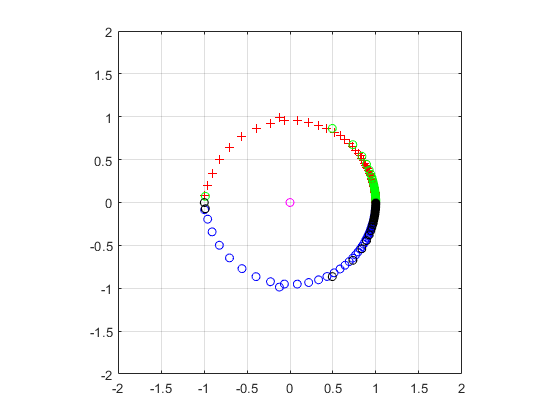
\includegraphics[scale=0.6]{images/radius.png}
    \caption{Eigenvalues of the amplification matrix in the complex plane}
    \label{fig:eigenval_amp}
\end{figure}
As we can observe on figure \ref{fig:eigenval_amp}, the eigenvalues of the amplification matrix $H(h)$ for different values of $h$ remain in the unit circle. When $h$ increases the eigenvalues are positioned at the left of the unit circle. For small values of $h$ the eigenvalues are at the right. For more complex case including those where the attenuation function are not assumed constant this result holds. This result ensures that the temporal integration scheme , we developed is stable in time for the one dimensional PML. This result shows that the integration scheme derived from the equation of the PML is stable in time. \\
In order to evaluate the properties of a numerical scheme in terms of stability, an interesting method is to look at the spectral radius, the periodicity error and the numerical damping. The spectral radius of the method is given by the modulus of the highest eigenvalue:
\begin{equation}
    R(A) = \max_i(|\lambda_i|)
\end{equation}
We will express this parameter in function of $\Omega = \omega h$ where $\omega = \sqrt{\frac{k}{m}}$ and $k=\frac{E S}{L_p}$. $m$ is the mass of the bar (in our case just an element). The asymptotic value of the spectral radius for $\omega h \rightarrow \infty$ gives an information about the stability of the method over the entire frequency domain.
\begin{figure}[H]
    \centering
    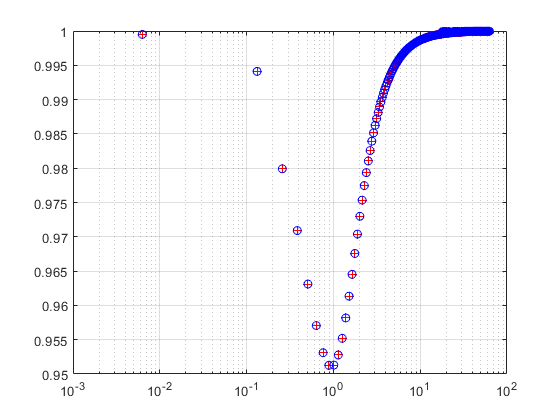
\includegraphics[scale=0.6]{images/spectral_rad.png}
    \caption{Spectral radius in function of $h\omega$}
    \label{fig:spectral_rad}
\end{figure}
As shown on the figure \ref{fig:spectral_rad}, the spectral radius remains under the value $1$ and its asymptotic value tends to $1$ as  $\omega h \rightarrow \infty$. This demonstrates that the numerical scheme is stable over the entire frequency domain. 
Let us now focus on the periodicity error which results from the comparison between the numerical and the exact frequencies obtained for the one degree-of-freedom oscillator:
\begin{equation}
    \frac{\Delta T}{T} = \frac{\omega h}{ \phi} - 1 \hspace{2cm}\textnormal{where} \hspace{1cm} \phi=tan^{-1}\left(\frac{\operatorname{Im} \lambda_1}{\operatorname{Re} \lambda_1}  \right)
    \label{eq:period_err}
\end{equation}
Therefore this is a measurement of the frequency distortion for each eigenfrequency in the model. 

\begin{figure}[H]
    \centering
    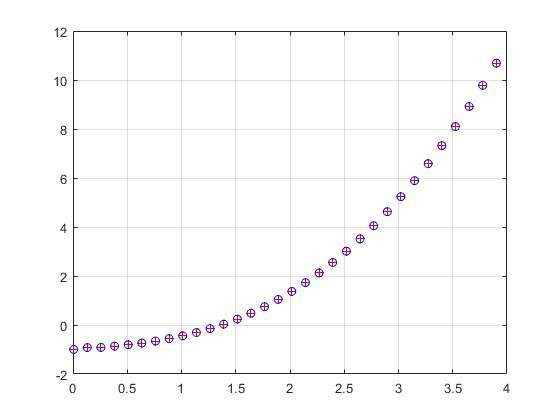
\includegraphics[scale=0.6]{images/relative_periodicity_error.png}
    \caption{relative periodicity error in function of $h\omega$}
    \label{fig:relative_per_err}
\end{figure}
As observed in \ref{fig:relative_per_err}, the relative periodicity error increases with $h \omega$ looking back at the equation \ref{eq:period_err} and knowing that the modulus of each eigenvalue is smaller or equal to $1$, the result obtained here about the relative periodicity error is the one expected. Since this result is difficult to interpret a more complete analysis will be done in the next report. Indeed some questions remain unanswered such as why the distortion at $h=0$ is different than $0$ or other questions about the numerical damping ratio we will present now. \\
The last parameter to be investigate is the numerical damping ratio. It compare the time decay coefficient of the real part of the solution to the numerical frequency.
\begin{equation}
    \xi = -\frac{log(|\lambda_1|)}{\phi}
    \label{eq:num_damp}
\end{equation}
It measures the percentage of critical damping introduced in the system by the integration operator. In fact it is expected to damped out the high frequencies introduced by the time integration operator.   
\begin{figure}[H]
    \centering
    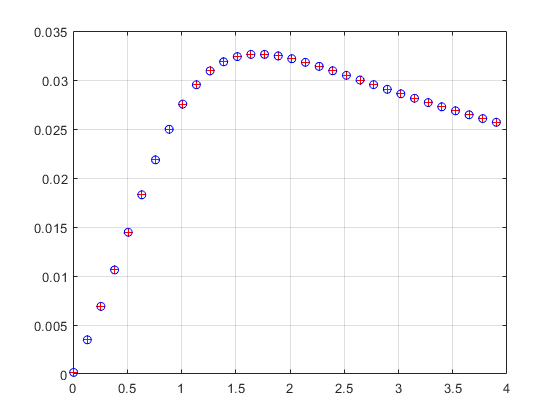
\includegraphics[scale=0.6]{images/Numerical_damping_ratio.png}
    \caption{Numerical damping ratio in function of $h\omega$}
    \label{fig:num_damp_ratio}
\end{figure}
In order to compare the results obtained on the Newmark-$\beta$ unconditionally stable scheme, let us make the same analysis of stability on the Newmark explicit temporal integration scheme for the PML with $\beta=0$ and $\alpha=0.5$ (central differences). 
\begin{figure}[H]
\centering
\begin{minipage}[b]{0.475\textwidth}
    \centering
    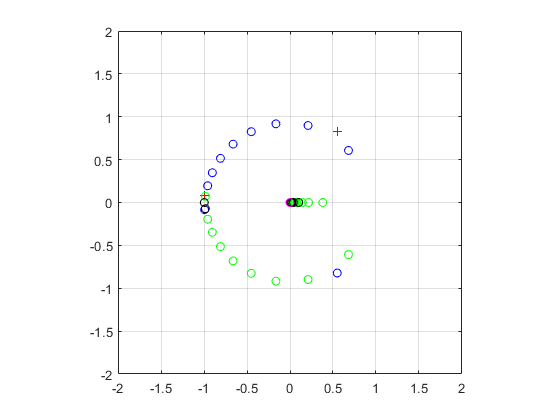
\includegraphics[width=\textwidth]{images/pml_expl_eig.png}
    \caption[Network2]%
    {{\small Eigenvalues in the complex plane}}    
    \label{fig:med_eig}
\end{minipage}
\hfill
\begin{minipage}[b]{0.475\textwidth}  
    \centering 
    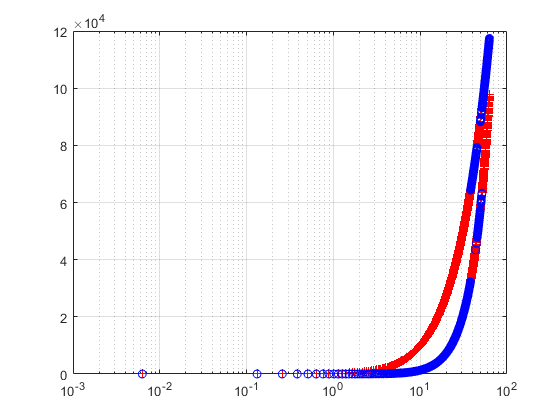
\includegraphics[width=\textwidth]{images/spectre_expl.png}
    \caption[]%
    {{\small Spectral radius in function of $h\omega$}}    
    \label{fig:med_spectre}
\end{minipage}
\vskip\baselineskip
\begin{minipage}[b]{0.475\textwidth}   
    \centering 
    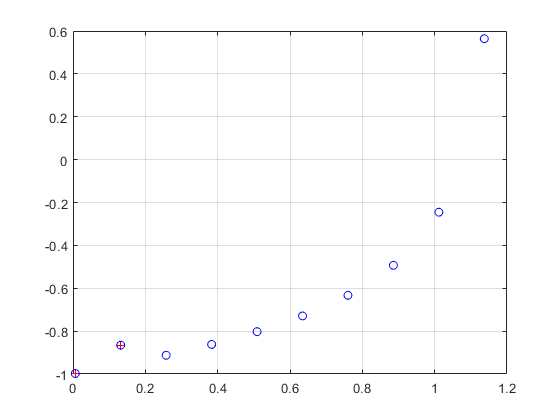
\includegraphics[width=\textwidth]{images/pml_exp_per.png}
    \caption[]%
    {{\small relative periodicity error in function of $h\omega$}}    
    \label{fig:med_relat_per}
\end{minipage}
\quad
\begin{minipage}[b]{0.475\textwidth}   
    \centering 
    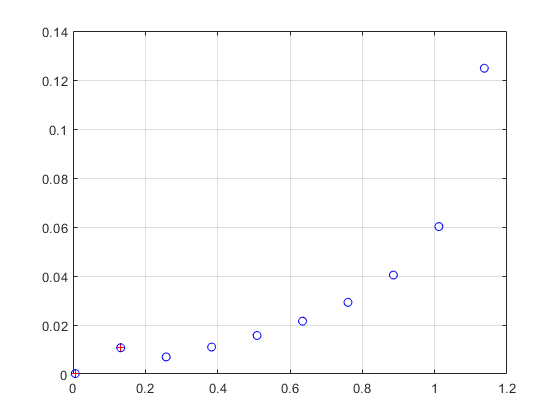
\includegraphics[width=\textwidth]{images/pml_expl_damp.png}
    \caption[]%
    {{\small Numerical damping ratio in function of $h\omega$}}    
    \label{fig:med_damp}
\end{minipage}
\end{figure}
As expected for a conditionally stable scheme, passed a certain value of $h \omega$ the scheme becomes unstable. This limit of stability is evaluated $h \omega = 2$ corresponding to the CFL condition.\\
We can also look at the behaviour of the Newmark explicit time integrator on the physical medium. In this case the equation of motion are the same as in a classic elastodynamic problem. In the following equation the state vector $q$ will be defined by $q^n=[\dot{u}^n, u^n]^T$. THe equation of motion at time $t^n$ and $t^{n+1}$ are:
\begin{equation}
\begin{aligned}
    M  \Ddot{u}^n &= -C \Dot{u}^n - K u^n +p^n  \\
    M \Ddot{u}^{n+1} &= -C \Dot{u}^{n+1} - K u^{n+1} +p^{n+1} 
\end{aligned}
\end{equation}
And taking into account the recurrence relationship given by the Newmark method:
\begin{equation}
\begin{aligned}
    M \dot{u}^{n+1} &= M\Dot{u}^{n} + h(1-\gamma)\left[ -C \Dot{u}^n - K u^n +p^n   \right] + \gamma h \left[ -C \Dot{u}^{n+1} - K u^{n+1} +p^{n+1} \right] \\
    M u^{n+1} &= M u^{n} + h M \dot{u}^n + h^2(\frac{1}{2}-\beta)\left[ -C \Dot{u}^n - K u^n +p^n   \right] + \beta h^2 \left[ -C \Dot{u}^{n+1} - K u^{n+1} +p^{n+1} \right]
\end{aligned}
\label{eq:med_rec}
\end{equation}
Therefore we can define the matrix form of this recurrence:
\begin{equation}
    q^{n+1} = A(h) q^n + g^{n+1}(h)
\end{equation}
The component of this relation can be defined using the equations \ref{eq:med_rec}. We obtain:
\begin{equation}
    A(h) = \begin{bmatrix}M+\gamma h C & \gamma h K \\ \beta h^2 C & M+ \beta h^2 K   \end{bmatrix}^{-1} \begin{bmatrix}(1-\gamma)hC-M& (1-\gamma)hK \\ (\frac{1}{2}-\beta)h^2C-hM& (\frac{1}{2}-\beta)h^2K-M \end{bmatrix} 
\end{equation}
and where
\begin{equation}
    g^{n+1}=\begin{bmatrix}M+\gamma h C & \gamma h K \\ \beta h^2 C & M+ \beta h^2 K   \end{bmatrix}^{-1} \begin{bmatrix}(1-\gamma)h p^n+\gamma h p^{n+1} \\ (\frac{1}{2}-\beta)h^2p^n+\beta h^2 p^{n+1}  \end{bmatrix}
\end{equation}
The matrix $A(h)$ is the matrix of amplification, its eigenvalues represents the normal vibration modes of the one dimensional element considered. Since the physical medium was assumed to have no damping $C=0$. Let us now expend the solution with respect to the eigenmodes of the structure. The equations of motion can be reduced to uncoupled normal equations:
\begin{equation}
    \Ddot{\eta}^n = - \omega \eta^n+\phi^n
\end{equation}
where $\phi^n$ is the participation factor at the excitation at time $t^n$. Thus using this system of uncoupled equations we can redifine the amplification matrix by:
\begin{equation}
    A(h) = \begin{bmatrix} 1& \gamma h \omega^2\\ 0&1+\beta h^2 \omega ^2\end{bmatrix}^{-1} \begin{bmatrix} 1& -(1-\gamma) h \omega^2\\ h&1-(\frac{1}{2}-\beta) h^2 \omega ^2\end{bmatrix}
\end{equation}
Using this definition of the amplification matrix, we can do the same analysis for the physical medium than the one done of the implicit Newmark scheme on the PML.
\begin{figure}[H]
\centering
\begin{minipage}[b]{0.475\textwidth}
    \centering
    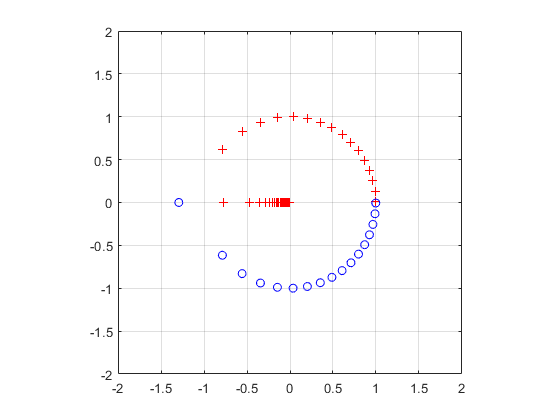
\includegraphics[width=\textwidth]{images/med_rad.png}
    \caption[Network2]%
    {{\small Eigenvalues in the complex plane}}    
    \label{fig:med_eig}
\end{minipage}
\hfill
\begin{minipage}[b]{0.475\textwidth}  
    \centering 
    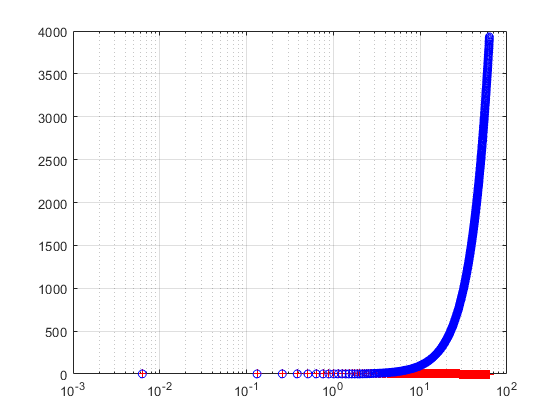
\includegraphics[width=\textwidth]{images/med_spectre.png}
    \caption[]%
    {{\small Spectral radius in function of $h\omega$}}    
    \label{fig:med_spectre}
\end{minipage}
\vskip\baselineskip
\begin{minipage}[b]{0.475\textwidth}   
    \centering 
    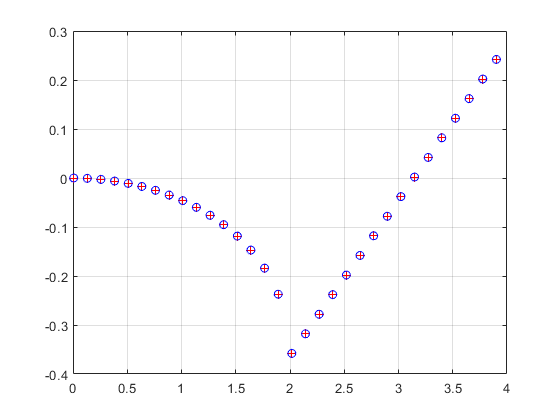
\includegraphics[width=\textwidth]{images/med_period.png}
    \caption[]%
    {{\small relative periodicity error in function of $h\omega$}}    
    \label{fig:med_relat_per}
\end{minipage}
\quad
\begin{minipage}[b]{0.475\textwidth}   
    \centering 
    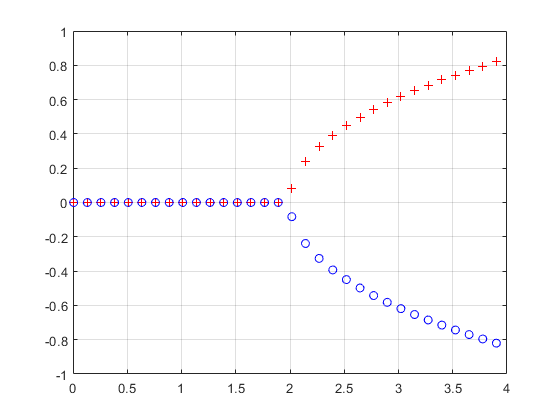
\includegraphics[width=\textwidth]{images/med_damp.png}
    \caption[]%
    {{\small Numerical damping ratio in function of $h\omega$}}    
    \label{fig:med_damp}
\end{minipage}
\end{figure}
We can observe on the figure \ref{fig:med_eig} that for a certain value of $h$ the eigenvalues seems to exit the unit circle. This is the proof that at a certain point the scheme becomes unstable and amplified drastically even small perturbations. This change from stable to unstable occurs when $h\omega > 2$ as we can see on the other figures






\newpage
\begin{frame}{Conclusion}
\begin{itemize}
\item Overview of the analysis of stability for integration method.
\item Stability of 1D and 2D perfectly matched layer (for implicit time integration method).
\item Properties of attenuation and delay of unstability for 1D PML.
\item \underline{Further work :}
\begin{itemize}
\item Same analysis of relative periodicity error and numerical damping for 2D PML.
\item Implementation of 2D Perfectly matched layer within Akantu. 
\end{itemize} 
\end{itemize}
\end{frame}


\newpage
%biblio
% Bibliographie
\bibliographystyle{plain}
\bibliography{biblio}
\end{document}
